\documentclass[10pt, etterpaper]{article}

\usepackage{times}
\usepackage{epsfig}
\usepackage{graphicx}
\usepackage{amsmath}
\usepackage{amssymb}


\usepackage{tikz}
\usepackage{soul}
\usetikzlibrary{shapes.misc, positioning, shapes.geometric, arrows}
\usepackage[a4paper,margin=1cm,landscape]{geometry}
\usetikzlibrary{positioning,shapes,shadows}


\tikzstyle{conv2d} = [rectangle, rounded corners, minimum width=4cm, minimum height=1cm,text centered, draw=black, fill=green!30]
\tikzstyle{bn} = [rectangle, rounded corners, minimum width=4cm, minimum height=1cm,text centered, draw=black, fill=red!30]
\tikzstyle{relu} = [rectangle, rounded corners, minimum width=4cm, minimum height=1cm,text centered, draw=black, fill=blue!30]
\tikzstyle{add} = [circle, radius=1cm,text centered, draw=black]
\tikzstyle{arrow} = [thick,->,>=stealth]
\tikzstyle{downsample} = [rectangle, minimum width=6cm, minimum height=4cm,text centered, draw=black, fill=yellow!30]
\tikzstyle{maxpool} = [rectangle, rounded corners, minimum width=4cm, minimum height=1cm,text centered, draw=black, fill=gray!30]

\tikzstyle{bt_ds} = [rectangle, rounded corners, minimum width=4cm, minimum height=1cm,text centered, draw=black, fill=orange!30]

\tikzstyle{bt_nods} = [rectangle, rounded corners, minimum width=4cm, minimum height=1cm,text centered, draw=black, fill=violet!30]

\def\ttx{1.4}

\setcounter{page}{1}
\begin{document}
\title{Deep Learning Architectures}

\author{Mohsen Kiskani}

\maketitle

%\begin{abstract}
%\end{abstract}

\section{Description}
\subsection{Basic Formulas}

\begin{align}
&\mathrm{Conv2D}(C_i, C_o, K, S=1, P=0, d=1) \\
&\mathrm{MaxPool2D}(K,S=None,P=0,d=1) \\
&\textrm{MaxPool2d and Conv2D}  \to L_{out} =  \lfloor  \frac{L_{in}+2P-d(K-1)-1}{S}+1\rfloor \\
&\mathrm{Conv2D}(C_i, C_o,1) \to L_{out} = L_{in} \\
&\mathrm{Conv2D}(C_i, C_o,3,1,1) \to L_{out} = L_{in} \\
&\textrm{Tensor representation} \to N \times C \times H \times W
\end{align}
%\section{Bottleneck}
%\label{sec_bottle}
\begin{figure}
\centering
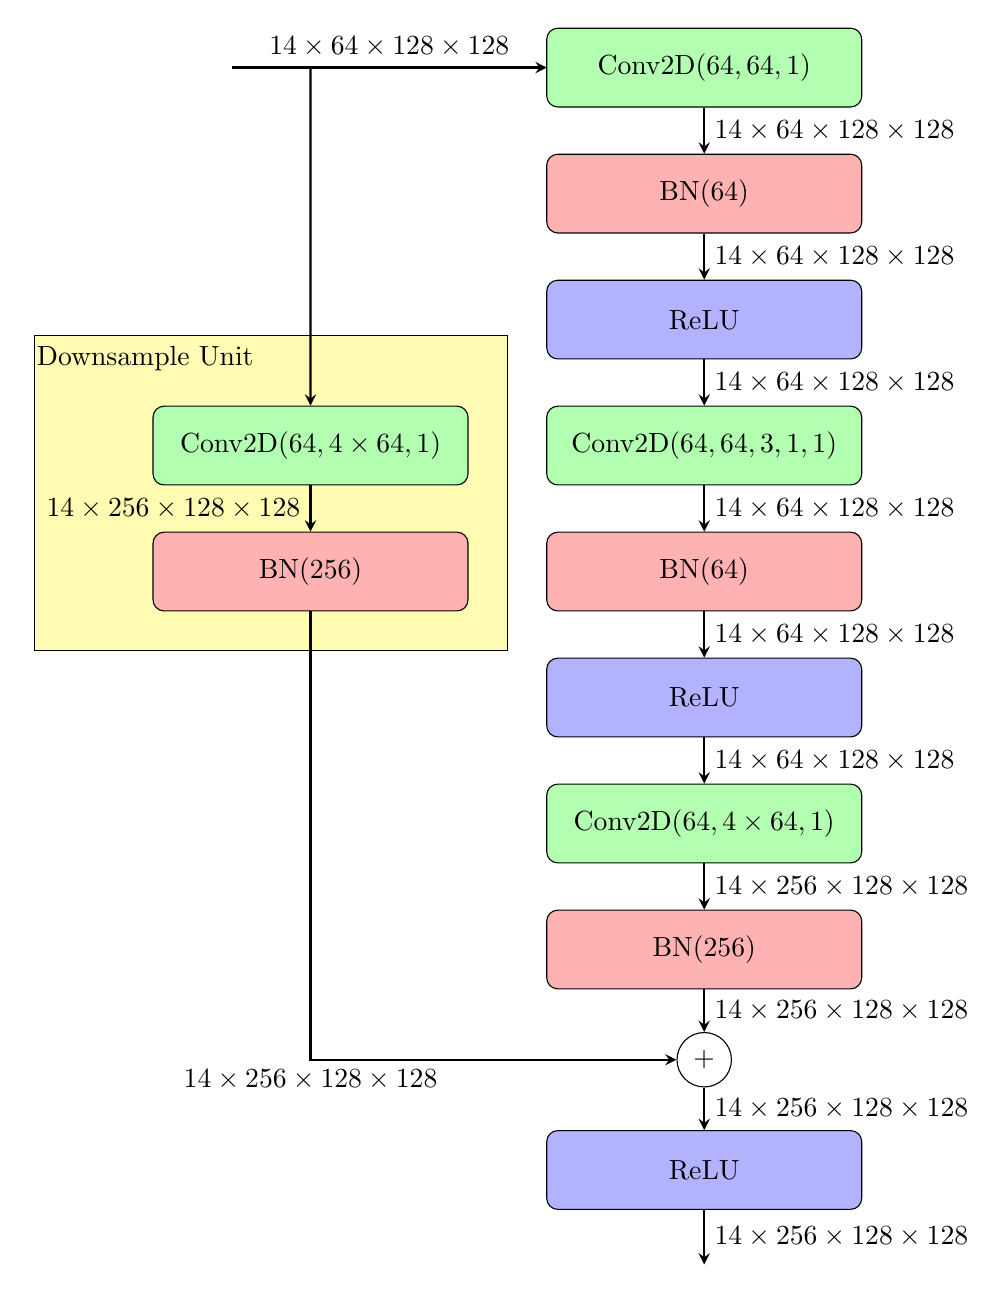
\begin{tikzpicture}[node distance=3cm]
\draw [arrow] (-6,0) -- node[anchor=south] {$14 \times 64 \times 128 \times 128$} (-2,0);

\node (conv1) [conv2d] {Conv2D$(64, 64, 1)$};
\node (bn1) [bn, below of= conv1, yshift=\ttx cm, xshift = 0cm] {BN($64$)};
\draw [arrow] (conv1) -- node[anchor=west]  {$14 \times 64 \times 128 \times 128$}  (bn1);
\node (relu1) [relu, below of= bn1, yshift=\ttx cm, xshift = 0cm] {ReLU};
\draw [arrow] (bn1) -- node[anchor=west]  {$14 \times 64 \times 128 \times 128$}  (relu1);

\node (conv2) [conv2d,  below of= relu1, yshift=\ttx cm, xshift = 0cm] {Conv2D$(64, 64, 3,1,1)$};
\draw [arrow] (relu1) -- node[anchor=west]  {$14 \times 64 \times 128 \times 128$}  (conv2);
\node (bn2) [bn, below of= conv2, yshift=\ttx cm, xshift = 0cm] {BN($64$)};
\draw [arrow] (conv2) -- node[anchor=west]  {$14 \times 64 \times 128 \times 128$}  (bn2);
\node (relu2) [relu, below of= bn2, yshift=\ttx cm, xshift = 0cm] {ReLU};
\draw [arrow] (bn2) -- node[anchor=west]  {$14 \times 64 \times 128 \times 128$}  (relu2);

\node (conv3) [conv2d, below of= relu2, yshift=\ttx cm, xshift = 0cm] {Conv2D$(64, 4 \times 64, 1)$};
\draw [arrow] (relu2) -- node[anchor=west]  {$14 \times 64 \times 128 \times 128$}  (conv3);
\node (bn3) [bn, below of= conv3, yshift=\ttx cm, xshift = 0cm] {BN($256$)};
\draw [arrow] (conv3) -- node[anchor=west]  {$14 \times 256 \times 128 \times 128$}  (bn3);
\node (sum) [add, below of=bn3,  yshift=1.6 cm, xshift = 0cm] {+};
\draw [arrow] (bn3) -- node[anchor=west]  {$14 \times 256 \times 128 \times 128$}  (sum);

\node (relu3) [relu, below of= sum, yshift=1.6 cm, xshift = 0cm] {ReLU};

\node (downsample) [downsample, left of = bn2, yshift=1 cm, xshift = -2.5cm] {};
\node [ yshift=-3.7 cm, xshift = -7.1cm] {Downsample Unit};


\node (conv4) [conv2d,  left of= conv2, yshift=0 cm, xshift = -2cm] {Conv2D$(64, 4 \times 64, 1)$};
\node (bn4) [bn, below of= conv4, yshift=\ttx cm, xshift = 0cm] {BN($256$)};
\draw [arrow] (-5,0) --  node[anchor=east] {} (conv4); %{$14 \times 64 \times 128 \times 128$}
\draw [arrow] (bn4) |-  node[anchor=north] {$14 \times 256 \times 128 \times 128$} (sum); %{$14 \times 64 \times 128 \times 128$}\\
\draw [arrow] (conv4) --  node[anchor=east] {$14 \times 256 \times 128 \times 128$} (bn4); %{$14 \times 64 \times 128 \times 128$}

\draw [arrow] (relu3) --  node[anchor=west] {$14 \times 256 \times 128 \times 128$} (0, -15.2);
\draw [arrow] (sum) --  node[anchor=west] {$14 \times 256 \times 128 \times 128$} (relu3);

\end{tikzpicture}
\caption{Bottleneck layer 1 with downsample unit}
\label{fig_bottleneck1_ds}
\end{figure}

\begin{figure}
\centering
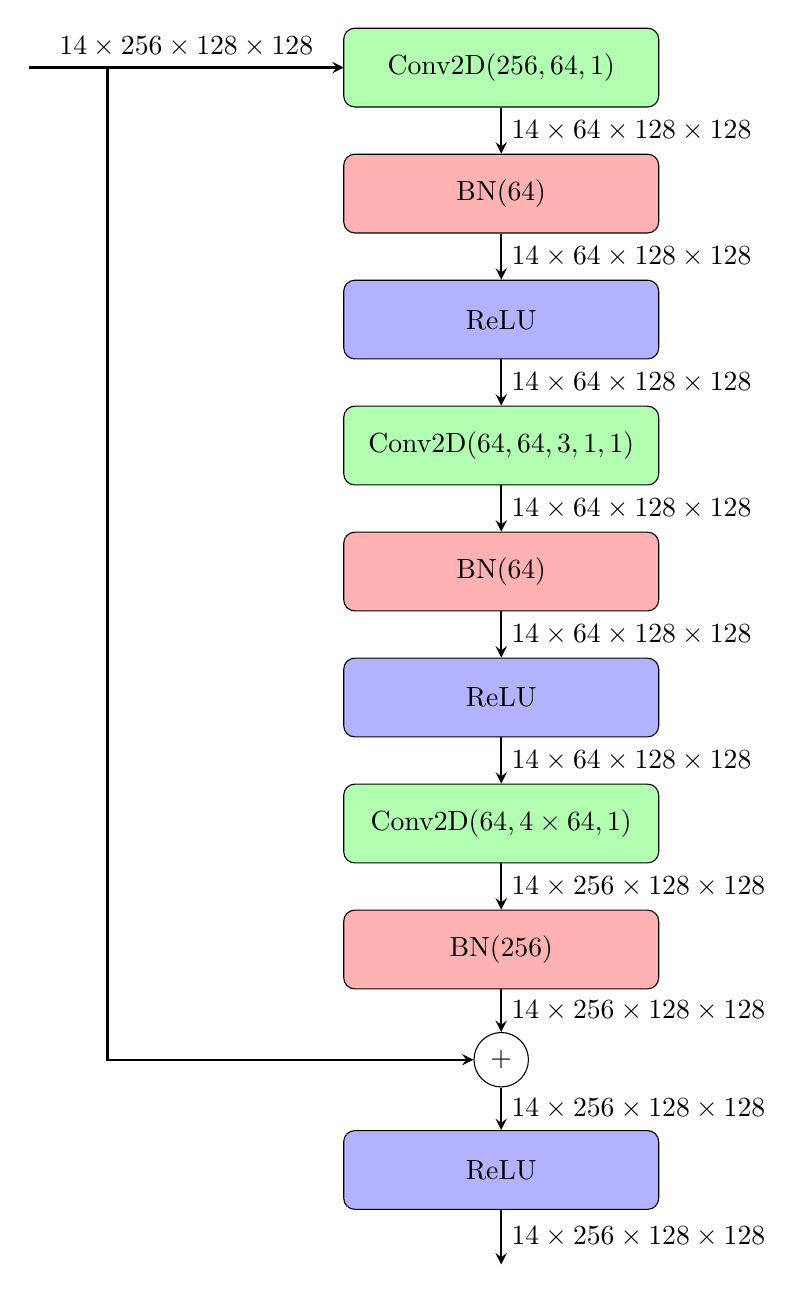
\begin{tikzpicture}[node distance=3cm]
\draw [arrow] (-6,0) -- node[anchor=south] {$14 \times 256 \times 128 \times 128$} (-2,0);

\node (conv1) [conv2d] {Conv2D$(256, 64, 1)$};
\node (bn1) [bn, below of= conv1, yshift=\ttx cm, xshift = 0cm] {BN($64$)};
\draw [arrow] (conv1) -- node[anchor=west]  {$14 \times 64 \times 128 \times 128$}  (bn1);
\node (relu1) [relu, below of= bn1, yshift=\ttx cm, xshift = 0cm] {ReLU};
\draw [arrow] (bn1) -- node[anchor=west]  {$14 \times 64 \times 128 \times 128$}  (relu1);

\node (conv2) [conv2d,  below of= relu1, yshift=\ttx cm, xshift = 0cm] {Conv2D$(64, 64, 3,1,1)$};
\draw [arrow] (relu1) -- node[anchor=west]  {$14 \times 64 \times 128 \times 128$}  (conv2);
\node (bn2) [bn, below of= conv2, yshift=\ttx cm, xshift = 0cm] {BN($64$)};
\draw [arrow] (conv2) -- node[anchor=west]  {$14 \times 64 \times 128 \times 128$}  (bn2);
\node (relu2) [relu, below of= bn2, yshift=\ttx cm, xshift = 0cm] {ReLU};
\draw [arrow] (bn2) -- node[anchor=west]  {$14 \times 64 \times 128 \times 128$}  (relu2);

\node (conv3) [conv2d, below of= relu2, yshift=\ttx cm, xshift = 0cm] {Conv2D$(64, 4 \times 64, 1)$};
\draw [arrow] (relu2) -- node[anchor=west]  {$14 \times 64 \times 128 \times 128$}  (conv3);
\node (bn3) [bn, below of= conv3, yshift=\ttx cm, xshift = 0cm] {BN($256$)};
\draw [arrow] (conv3) -- node[anchor=west]  {$14 \times 256 \times 128 \times 128$}  (bn3);
\node (sum) [add, below of=bn3,  yshift=1.6 cm, xshift = 0cm] {+};
\draw [arrow] (bn3) -- node[anchor=west]  {$14 \times 256 \times 128 \times 128$}  (sum);

\node (relu3) [relu, below of= sum, yshift=1.6 cm, xshift = 0cm] {ReLU};

\draw [arrow] (-5,0) |-  node[anchor=east] {} (sum); 

\draw [arrow] (relu3) --  node[anchor=west] {$14 \times 256 \times 128 \times 128$} (0, -15.2);
\draw [arrow] (sum) --  node[anchor=west] {$14 \times 256 \times 128 \times 128$} (relu3);

\end{tikzpicture}
\caption{Bottleneck layer 1 without downsample unit}
\label{fig_bottleneck1_nods}
\end{figure}




\begin{figure}
\centering
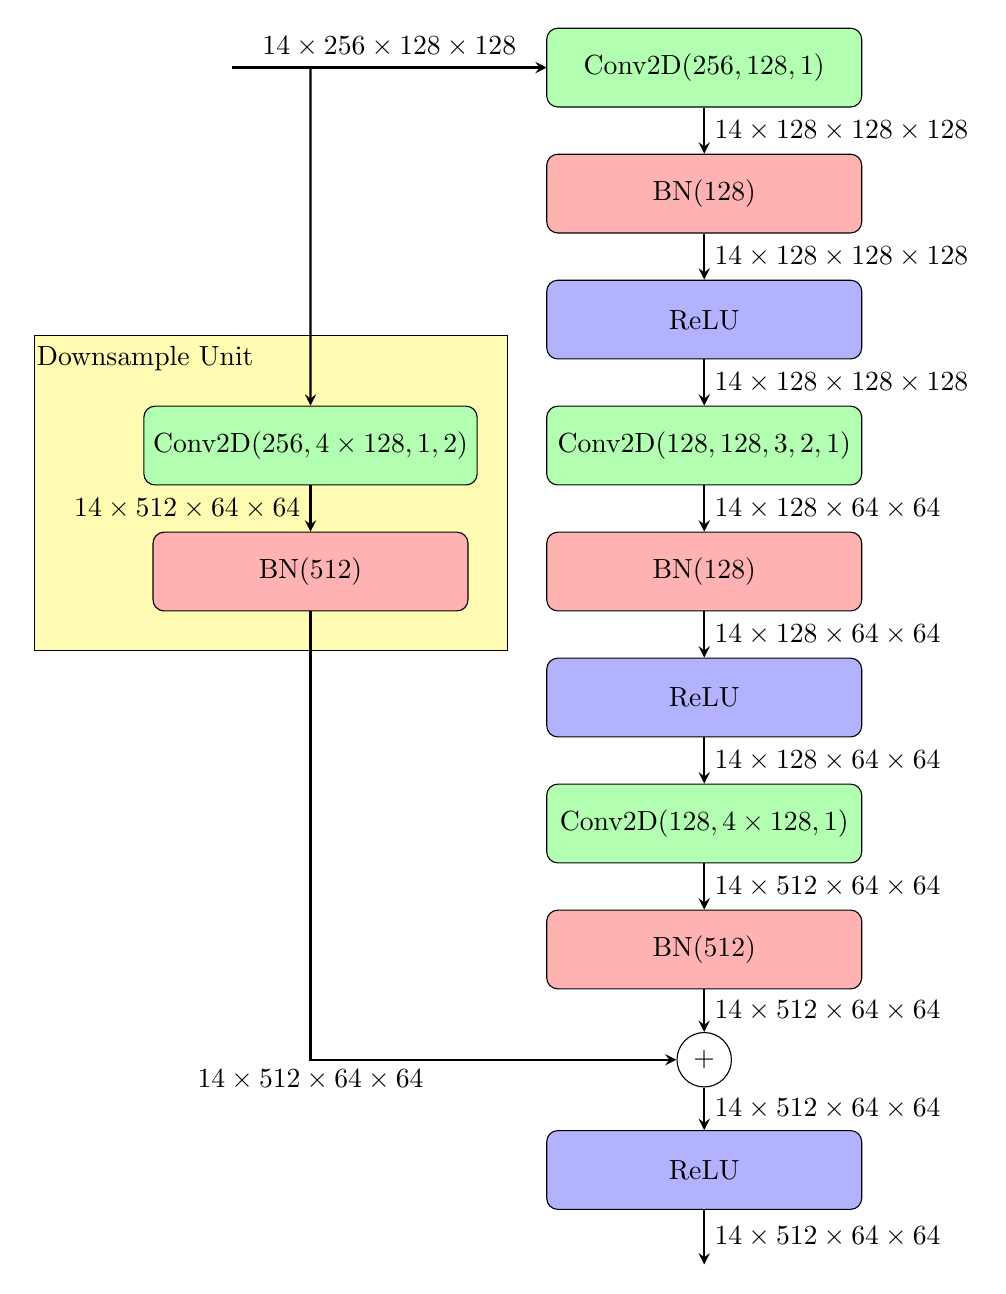
\begin{tikzpicture}[node distance=3cm]
\draw [arrow] (-6,0) -- node[anchor=south] {$14 \times 256 \times 128 \times 128$} (-2,0);

\node (conv1) [conv2d] {Conv2D$(256, 128, 1)$};
\node (bn1) [bn, below of= conv1, yshift=\ttx cm, xshift = 0cm] {BN($128$)};
\draw [arrow] (conv1) -- node[anchor=west]  {$14 \times 128 \times 128 \times 128$}  (bn1);
\node (relu1) [relu, below of= bn1, yshift=\ttx cm, xshift = 0cm] {ReLU};
\draw [arrow] (bn1) -- node[anchor=west]  {$14 \times 128 \times 128 \times 128$}  (relu1);

\node (conv2) [conv2d,  below of= relu1, yshift=\ttx cm, xshift = 0cm] {Conv2D$(128, 128, 3,2,1)$};
\draw [arrow] (relu1) -- node[anchor=west]  {$14 \times 128 \times 128 \times 128$}  (conv2);
\node (bn2) [bn, below of= conv2, yshift=\ttx cm, xshift = 0cm] {BN($128$)};
\draw [arrow] (conv2) -- node[anchor=west]  {$14 \times 128 \times 64 \times 64$}  (bn2);
\node (relu2) [relu, below of= bn2, yshift=\ttx cm, xshift = 0cm] {ReLU};
\draw [arrow] (bn2) -- node[anchor=west]  {$14 \times 128 \times 64 \times 64$}  (relu2);

\node (conv3) [conv2d, below of= relu2, yshift=\ttx cm, xshift = 0cm] {Conv2D$(128, 4 \times 128, 1)$};
\draw [arrow] (relu2) -- node[anchor=west]  {$14 \times 128 \times 64 \times 64$}  (conv3);
\node (bn3) [bn, below of= conv3, yshift=\ttx cm, xshift = 0cm] {BN($512$)};
\draw [arrow] (conv3) -- node[anchor=west]  {$14 \times 512 \times 64 \times 64$}  (bn3);
\node (sum) [add, below of=bn3,  yshift=1.6 cm, xshift = 0cm] {+};
\draw [arrow] (bn3) -- node[anchor=west]  {$14 \times 512 \times 64 \times 64$}  (sum);

\node (relu3) [relu, below of= sum, yshift=1.6 cm, xshift = 0cm] {ReLU};

\node (downsample) [downsample, left of = bn2, yshift=1 cm, xshift = -2.5cm] {};
\node [ yshift=-3.7 cm, xshift = -7.1cm] {Downsample Unit};


\node (conv4) [conv2d,  left of= conv2, yshift=0 cm, xshift = -2cm] {Conv2D$(256, 4 \times 128, 1, 2)$};
\node (bn4) [bn, below of= conv4, yshift=\ttx cm, xshift = 0cm] {BN($512$)};
\draw [arrow] (-5,0) --  node[anchor=east] {} (conv4); %{$14 \times 64 \times 128 \times 128$}
\draw [arrow] (bn4) |-  node[anchor=north] {$14 \times 512 \times 64 \times 64$} (sum); %{$14 \times 64 \times 128 \times 128$}\\
\draw [arrow] (conv4) --  node[anchor=east] {$14 \times 512 \times 64 \times 64$} (bn4); %{$14 \times 64 \times 128 \times 128$}

\draw [arrow] (relu3) --  node[anchor=west] {$14 \times 512 \times 64 \times 64$} (0, -15.2);
\draw [arrow] (sum) --  node[anchor=west] {$14 \times 512 \times 64 \times 64$} (relu3);

\end{tikzpicture}
\caption{Bottleneck layer 2 with downsample unit}
\label{fig_bottleneck2_ds}
\end{figure}



\begin{figure}
\centering
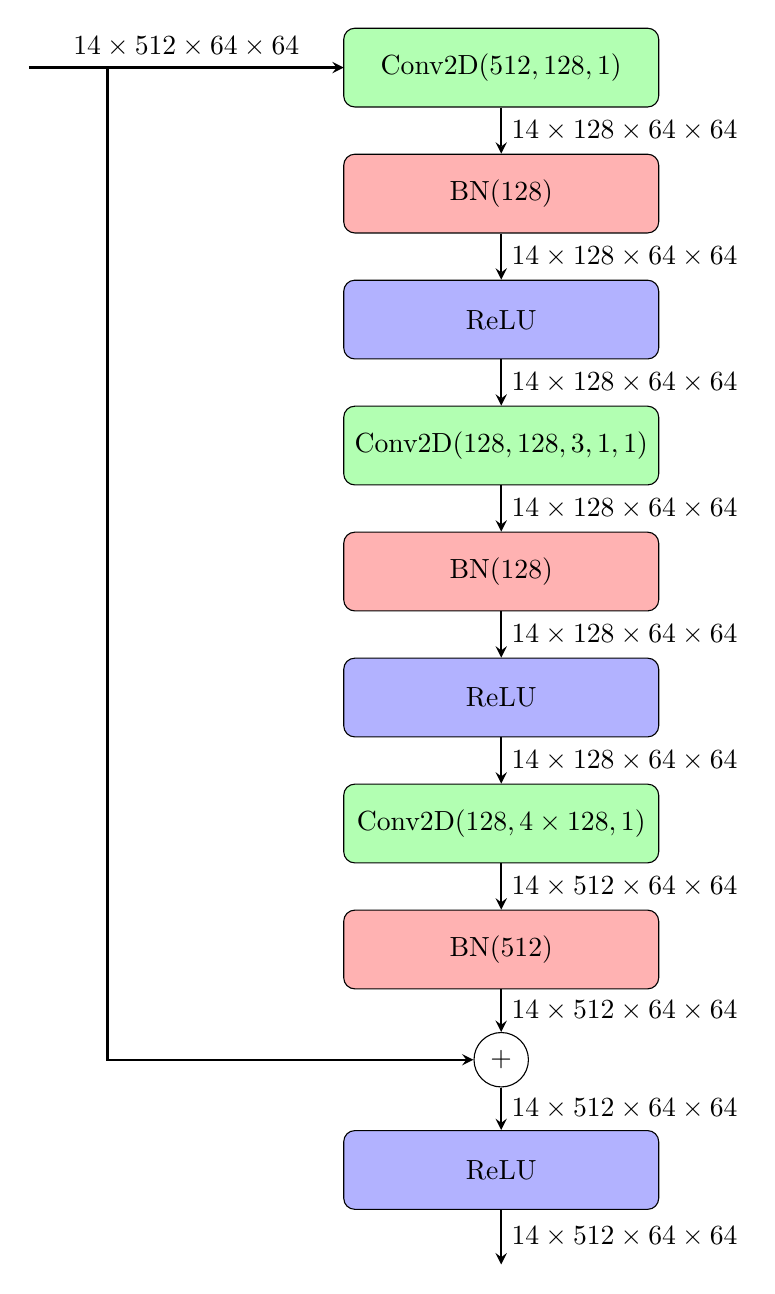
\begin{tikzpicture}[node distance=3cm]
\draw [arrow] (-6,0) -- node[anchor=south] {$14 \times 512 \times 64 \times 64$} (-2,0);

\node (conv1) [conv2d] {Conv2D$(512, 128, 1)$};
\node (bn1) [bn, below of= conv1, yshift=\ttx cm, xshift = 0cm] {BN($128$)};
\draw [arrow] (conv1) -- node[anchor=west]  {$14 \times 128 \times 64 \times 64$}  (bn1);
\node (relu1) [relu, below of= bn1, yshift=\ttx cm, xshift = 0cm] {ReLU};
\draw [arrow] (bn1) -- node[anchor=west]  {$14 \times 128 \times 64 \times 64$}  (relu1);

\node (conv2) [conv2d,  below of= relu1, yshift=\ttx cm, xshift = 0cm] {Conv2D$(128, 128, 3,1,1)$};
\draw [arrow] (relu1) -- node[anchor=west]  {$14 \times 128 \times 64 \times 64$}  (conv2);
\node (bn2) [bn, below of= conv2, yshift=\ttx cm, xshift = 0cm] {BN($128$)};
\draw [arrow] (conv2) -- node[anchor=west]  {$14 \times 128 \times 64 \times 64$}  (bn2);
\node (relu2) [relu, below of= bn2, yshift=\ttx cm, xshift = 0cm] {ReLU};
\draw [arrow] (bn2) -- node[anchor=west]  {$14 \times 128 \times 64 \times 64$}  (relu2);

\node (conv3) [conv2d, below of= relu2, yshift=\ttx cm, xshift = 0cm] {Conv2D$(128, 4 \times 128, 1)$};
\draw [arrow] (relu2) -- node[anchor=west]  {$14 \times 128 \times 64 \times 64$}  (conv3);
\node (bn3) [bn, below of= conv3, yshift=\ttx cm, xshift = 0cm] {BN($512$)};
\draw [arrow] (conv3) -- node[anchor=west]  {$14 \times 512 \times 64 \times 64$}  (bn3);
\node (sum) [add, below of=bn3,  yshift=1.6 cm, xshift = 0cm] {+};
\draw [arrow] (bn3) -- node[anchor=west]  {$14 \times 512 \times 64 \times 64$}  (sum);

\node (relu3) [relu, below of= sum, yshift=1.6 cm, xshift = 0cm] {ReLU};

\draw [arrow] (-5,0) |-  node[anchor=east] {} (sum); 

\draw [arrow] (relu3) --  node[anchor=west] {$14 \times 512 \times 64 \times 64$} (0, -15.2);
\draw [arrow] (sum) --  node[anchor=west] {$14 \times 512 \times 64 \times 64$} (relu3);

\end{tikzpicture}
\caption{Bottleneck layer 2 without downsample unit}
\label{fig_bottleneck2_nods}
\end{figure}






\begin{figure}
\centering
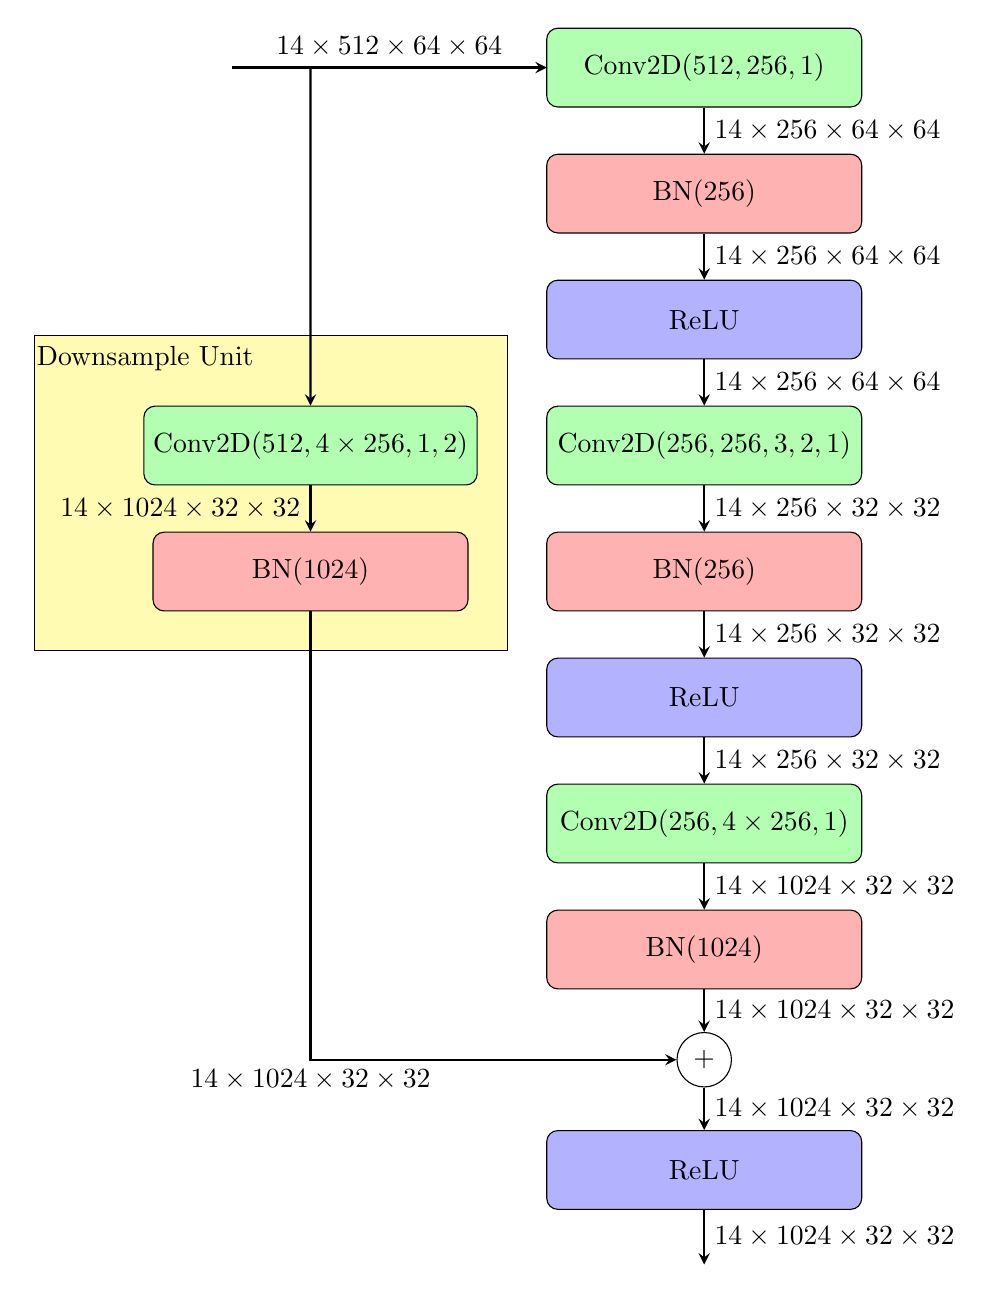
\begin{tikzpicture}[node distance=3cm]
\draw [arrow] (-6,0) -- node[anchor=south] {$14 \times 512 \times 64 \times 64$} (-2,0);

\node (conv1) [conv2d] {Conv2D$(512, 256, 1)$};
\node (bn1) [bn, below of= conv1, yshift=\ttx cm, xshift = 0cm] {BN($256$)};
\draw [arrow] (conv1) -- node[anchor=west]  {$14 \times 256 \times 64 \times 64$}  (bn1);
\node (relu1) [relu, below of= bn1, yshift=\ttx cm, xshift = 0cm] {ReLU};
\draw [arrow] (bn1) -- node[anchor=west]  {$14 \times 256  \times 64 \times 64$}  (relu1);

\node (conv2) [conv2d,  below of= relu1, yshift=\ttx cm, xshift = 0cm] {Conv2D$(256, 256, 3,2,1)$};
\draw [arrow] (relu1) -- node[anchor=west]  {$14 \times 256 \times 64 \times 64$}  (conv2);
\node (bn2) [bn, below of= conv2, yshift=\ttx cm, xshift = 0cm] {BN($256$)};
\draw [arrow] (conv2) -- node[anchor=west]  {$14 \times 256 \times 32 \times 32$}  (bn2);
\node (relu2) [relu, below of= bn2, yshift=\ttx cm, xshift = 0cm] {ReLU};
\draw [arrow] (bn2) -- node[anchor=west]  {$14 \times 256 \times 32 \times 32$}  (relu2);

\node (conv3) [conv2d, below of= relu2, yshift=\ttx cm, xshift = 0cm] {Conv2D$(256, 4 \times 256, 1)$};
\draw [arrow] (relu2) -- node[anchor=west]  {$14 \times 256 \times 32 \times 32$}  (conv3);
\node (bn3) [bn, below of= conv3, yshift=\ttx cm, xshift = 0cm] {BN($1024$)};
\draw [arrow] (conv3) -- node[anchor=west]  {$14 \times 1024 \times 32 \times 32$}  (bn3);
\node (sum) [add, below of=bn3,  yshift=1.6 cm, xshift = 0cm] {+};
\draw [arrow] (bn3) -- node[anchor=west]  {$14 \times 1024 \times 32 \times 32$}  (sum);

\node (relu3) [relu, below of= sum, yshift=1.6 cm, xshift = 0cm] {ReLU};

\node (downsample) [downsample, left of = bn2, yshift=1 cm, xshift = -2.5cm] {};
\node [ yshift=-3.7 cm, xshift = -7.1cm] {Downsample Unit};


\node (conv4) [conv2d,  left of= conv2, yshift=0 cm, xshift = -2cm] {Conv2D$(512, 4 \times 256, 1, 2)$};
\node (bn4) [bn, below of= conv4, yshift=\ttx cm, xshift = 0cm] {BN($1024$)};
\draw [arrow] (-5,0) --  node[anchor=east] {} (conv4); %{$14 \times 64 \times 128 \times 128$}
\draw [arrow] (bn4) |-  node[anchor=north] {$14 \times 1024 \times 32 \times 32$} (sum);  
\draw [arrow] (conv4) --  node[anchor=east] {$14 \times 1024 \times 32 \times 32$} (bn4);  

\draw [arrow] (relu3) --  node[anchor=west] {$14 \times 1024 \times 32 \times 32$} (0, -15.2);
\draw [arrow] (sum) --  node[anchor=west] {$14 \times 1024 \times 32 \times 32$} (relu3);

\end{tikzpicture}
\caption{Bottleneck layer 3 with downsample unit}
\label{fig_bottleneck3_ds}
\end{figure}



\begin{figure}
\centering
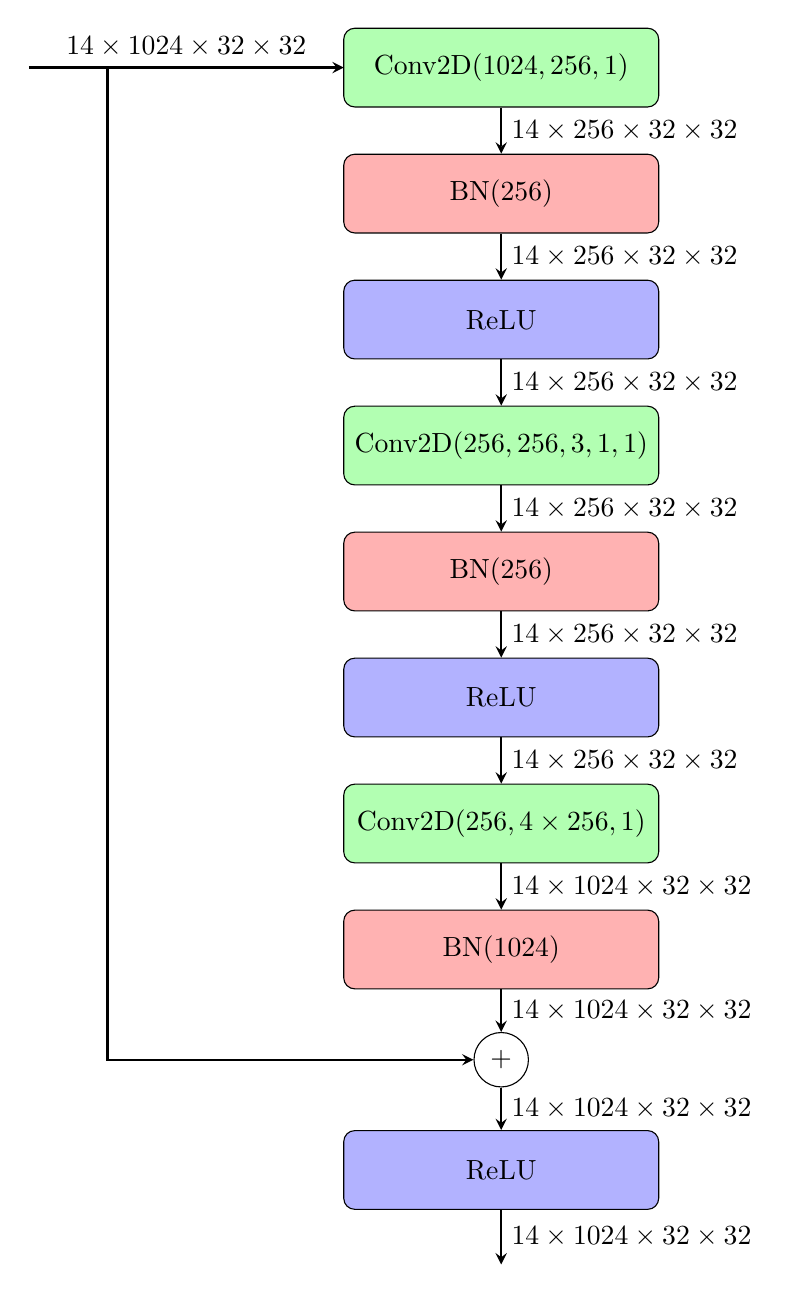
\begin{tikzpicture}[node distance=3cm]
\draw [arrow] (-6,0) -- node[anchor=south] {$14 \times 1024 \times 32 \times 32$} (-2,0);

\node (conv1) [conv2d] {Conv2D$(1024, 256, 1)$};
\node (bn1) [bn, below of= conv1, yshift=\ttx cm, xshift = 0cm] {BN($256$)};
\draw [arrow] (conv1) -- node[anchor=west]  {$14 \times 256 \times 32 \times 32$}  (bn1);
\node (relu1) [relu, below of= bn1, yshift=\ttx cm, xshift = 0cm] {ReLU};
\draw [arrow] (bn1) -- node[anchor=west]  {$14 \times 256 \times 32 \times 32$}  (relu1);

\node (conv2) [conv2d,  below of= relu1, yshift=\ttx cm, xshift = 0cm] {Conv2D$(256, 256, 3,1,1)$};
\draw [arrow] (relu1) -- node[anchor=west]  {$14 \times 256 \times 32 \times 32$}  (conv2);
\node (bn2) [bn, below of= conv2, yshift=\ttx cm, xshift = 0cm] {BN($256$)};
\draw [arrow] (conv2) -- node[anchor=west]  {$14 \times 256 \times 32 \times 32$}  (bn2);
\node (relu2) [relu, below of= bn2, yshift=\ttx cm, xshift = 0cm] {ReLU};
\draw [arrow] (bn2) -- node[anchor=west]  {$14 \times 256 \times 32 \times 32$}  (relu2);

\node (conv3) [conv2d, below of= relu2, yshift=\ttx cm, xshift = 0cm] {Conv2D$(256, 4 \times 256, 1)$};
\draw [arrow] (relu2) -- node[anchor=west]  {$14 \times 256 \times 32 \times 32$}  (conv3);
\node (bn3) [bn, below of= conv3, yshift=\ttx cm, xshift = 0cm] {BN($1024$)};
\draw [arrow] (conv3) -- node[anchor=west]  {$14 \times 1024 \times 32 \times 32$}  (bn3);
\node (sum) [add, below of=bn3,  yshift=1.6 cm, xshift = 0cm] {+};
\draw [arrow] (bn3) -- node[anchor=west]  {$14 \times 1024 \times 32 \times 32$}  (sum);

\node (relu3) [relu, below of= sum, yshift=1.6 cm, xshift = 0cm] {ReLU};

\draw [arrow] (-5,0) |-  node[anchor=east] {} (sum); 

\draw [arrow] (relu3) --  node[anchor=west] {$14 \times 1024 \times 32 \times 32$} (0, -15.2);
\draw [arrow] (sum) --  node[anchor=west] {$14 \times 1024 \times 32 \times 32$} (relu3);

\end{tikzpicture}
\caption{Bottleneck layer 3 without downsample unit}
\label{fig_bottleneck3_nods}
\end{figure}





\begin{figure}
\centering
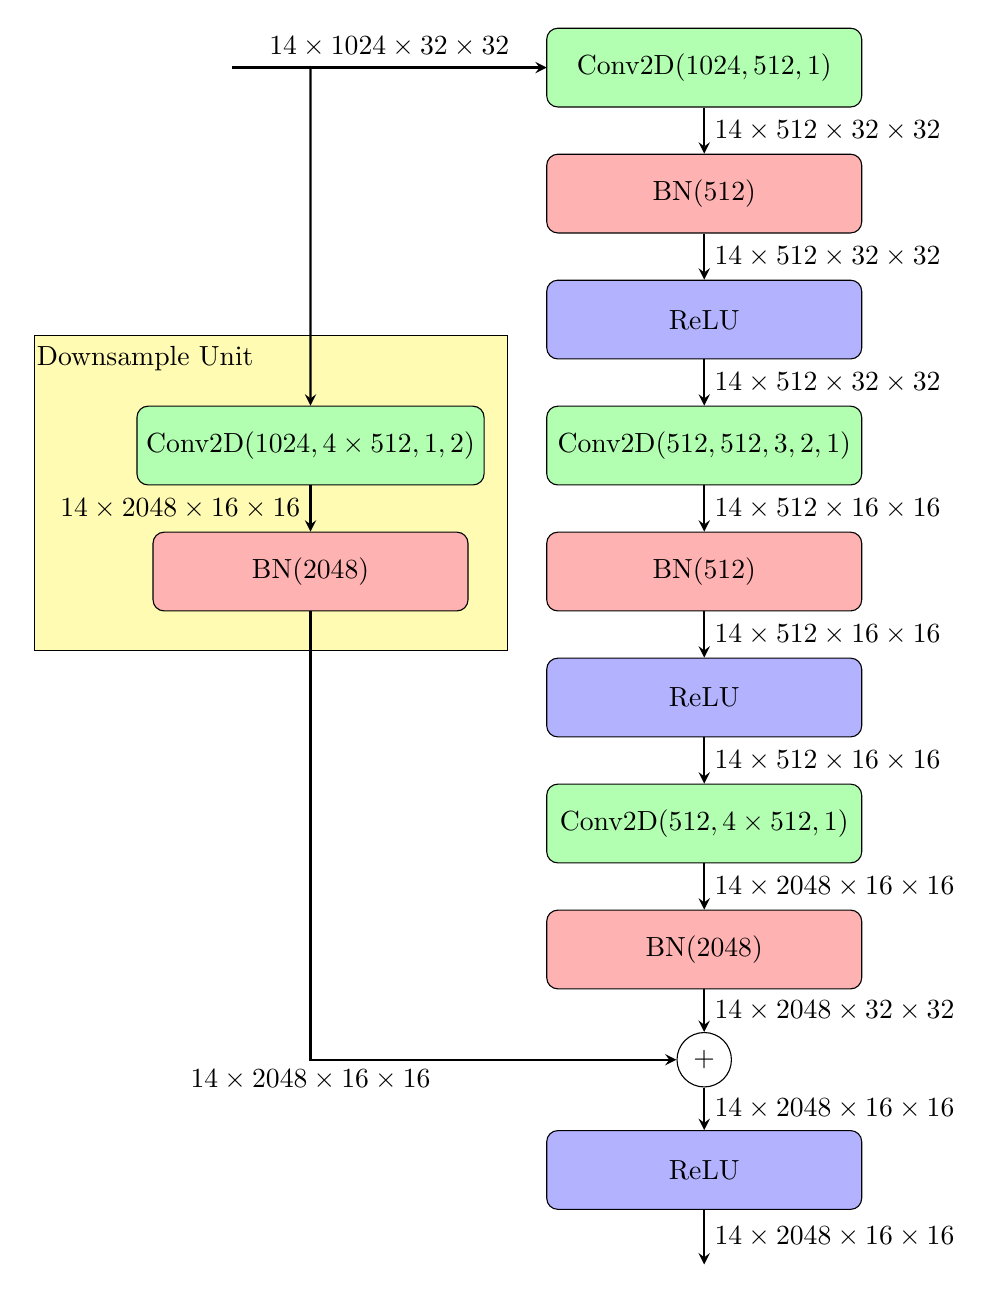
\begin{tikzpicture}[node distance=3cm]
\draw [arrow] (-6,0) -- node[anchor=south] {$14 \times 1024 \times 32 \times 32$} (-2,0);

\node (conv1) [conv2d] {Conv2D$(1024, 512, 1)$};
\node (bn1) [bn, below of= conv1, yshift=\ttx cm, xshift = 0cm] {BN($512$)};
\draw [arrow] (conv1) -- node[anchor=west]  {$14 \times 512 \times 32 \times 32$}  (bn1);
\node (relu1) [relu, below of= bn1, yshift=\ttx cm, xshift = 0cm] {ReLU};
\draw [arrow] (bn1) -- node[anchor=west]  {$14 \times 512  \times 32 \times 32$}  (relu1);

\node (conv2) [conv2d,  below of= relu1, yshift=\ttx cm, xshift = 0cm] {Conv2D$(512, 512, 3,2,1)$};
\draw [arrow] (relu1) -- node[anchor=west]  {$14 \times 512 \times 32 \times 32$}  (conv2);
\node (bn2) [bn, below of= conv2, yshift=\ttx cm, xshift = 0cm] {BN($512$)};
\draw [arrow] (conv2) -- node[anchor=west]  {$14 \times 512 \times 16 \times 16$}  (bn2);
\node (relu2) [relu, below of= bn2, yshift=\ttx cm, xshift = 0cm] {ReLU};
\draw [arrow] (bn2) -- node[anchor=west]  {$14 \times 512 \times 16 \times 16$}  (relu2);

\node (conv3) [conv2d, below of= relu2, yshift=\ttx cm, xshift = 0cm] {Conv2D$(512, 4 \times 512, 1)$};
\draw [arrow] (relu2) -- node[anchor=west]  {$14 \times 512 \times 16 \times 16$}  (conv3);
\node (bn3) [bn, below of= conv3, yshift=\ttx cm, xshift = 0cm] {BN($2048$)};
\draw [arrow] (conv3) -- node[anchor=west]  {$14 \times 2048 \times 16 \times 16$}  (bn3);
\node (sum) [add, below of=bn3,  yshift=1.6 cm, xshift = 0cm] {+};
\draw [arrow] (bn3) -- node[anchor=west]  {$14 \times 2048 \times 32 \times 32$}  (sum);

\node (relu3) [relu, below of= sum, yshift=1.6 cm, xshift = 0cm] {ReLU};

\node (downsample) [downsample, left of = bn2, yshift=1 cm, xshift = -2.5cm] {};
\node [ yshift=-3.7 cm, xshift = -7.1cm] {Downsample Unit};


\node (conv4) [conv2d,  left of= conv2, yshift=0 cm, xshift = -2cm] {Conv2D$(1024, 4 \times 512, 1, 2)$};
\node (bn4) [bn, below of= conv4, yshift=\ttx cm, xshift = 0cm] {BN($2048$)};
\draw [arrow] (-5,0) --  node[anchor=east] {} (conv4); %{$14 \times 64 \times 128 \times 128$}
\draw [arrow] (bn4) |-  node[anchor=north] {$14 \times 2048 \times 16 \times 16$} (sum);  
\draw [arrow] (conv4) --  node[anchor=east] {$14 \times 2048 \times 16 \times 16$} (bn4);  

\draw [arrow] (relu3) --  node[anchor=west] {$14 \times 2048 \times 16 \times 16$} (0, -15.2);
\draw [arrow] (sum) --  node[anchor=west] {$14 \times 2048 \times 16 \times 16$} (relu3);

\end{tikzpicture}
\caption{Bottleneck layer 4 with downsample unit}
\label{fig_bottleneck4_ds}
\end{figure}



\begin{figure}
\centering
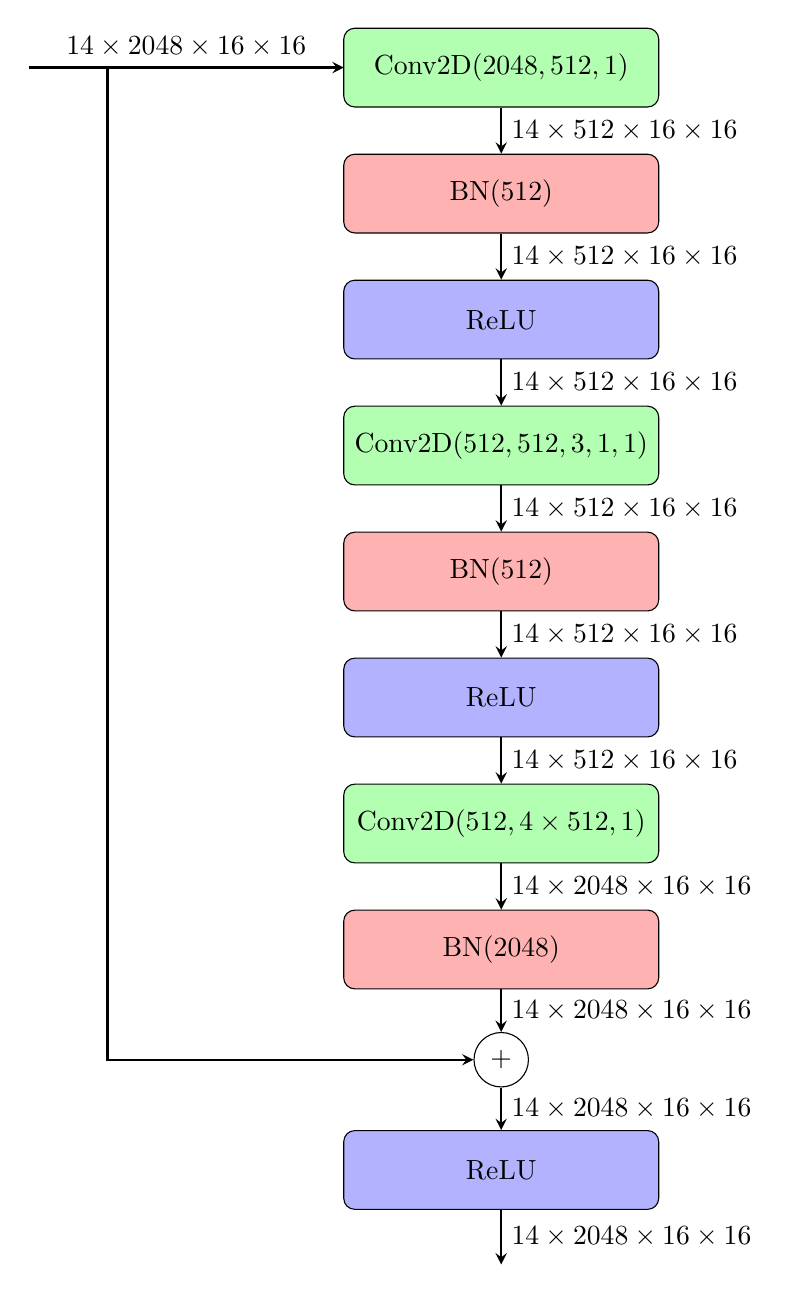
\begin{tikzpicture}[node distance=3cm]
\draw [arrow] (-6,0) -- node[anchor=south] {$14 \times 2048 \times 16 \times 16$} (-2,0);

\node (conv1) [conv2d] {Conv2D$(2048, 512, 1)$};
\node (bn1) [bn, below of= conv1, yshift=\ttx cm, xshift = 0cm] {BN($512$)};
\draw [arrow] (conv1) -- node[anchor=west]  {$14 \times 512 \times 16 \times 16$}  (bn1);
\node (relu1) [relu, below of= bn1, yshift=\ttx cm, xshift = 0cm] {ReLU};
\draw [arrow] (bn1) -- node[anchor=west]  {$14 \times 512 \times 16 \times 16$}  (relu1);

\node (conv2) [conv2d,  below of= relu1, yshift=\ttx cm, xshift = 0cm] {Conv2D$(512, 512, 3,1,1)$};
\draw [arrow] (relu1) -- node[anchor=west]  {$14 \times 512 \times 16 \times 16$}  (conv2);
\node (bn2) [bn, below of= conv2, yshift=\ttx cm, xshift = 0cm] {BN($512$)};
\draw [arrow] (conv2) -- node[anchor=west]  {$14 \times 512 \times 16 \times 16$}  (bn2);
\node (relu2) [relu, below of= bn2, yshift=\ttx cm, xshift = 0cm] {ReLU};
\draw [arrow] (bn2) -- node[anchor=west]  {$14 \times 512 \times 16 \times 16$}  (relu2);

\node (conv3) [conv2d, below of= relu2, yshift=\ttx cm, xshift = 0cm] {Conv2D$(512, 4 \times 512, 1)$};
\draw [arrow] (relu2) -- node[anchor=west]  {$14 \times 512 \times 16 \times 16$}  (conv3);
\node (bn3) [bn, below of= conv3, yshift=\ttx cm, xshift = 0cm] {BN($2048$)};
\draw [arrow] (conv3) -- node[anchor=west]  {$14 \times 2048 \times 16 \times 16$}  (bn3);
\node (sum) [add, below of=bn3,  yshift=1.6 cm, xshift = 0cm] {+};
\draw [arrow] (bn3) -- node[anchor=west]  {$14 \times 2048 \times 16 \times 16$}  (sum);

\node (relu3) [relu, below of= sum, yshift=1.6 cm, xshift = 0cm] {ReLU};

\draw [arrow] (-5,0) |-  node[anchor=east] {} (sum); 

\draw [arrow] (relu3) --  node[anchor=west] {$14 \times 2048 \times 16 \times 16$} (0, -15.2);
\draw [arrow] (sum) --  node[anchor=west] {$14 \times 2048 \times 16 \times 16$} (relu3);

\end{tikzpicture}
\caption{Bottleneck layer 4 without downsample unit}
\label{fig_bottleneck4_nods}
\end{figure}



\begin{figure}
\centering
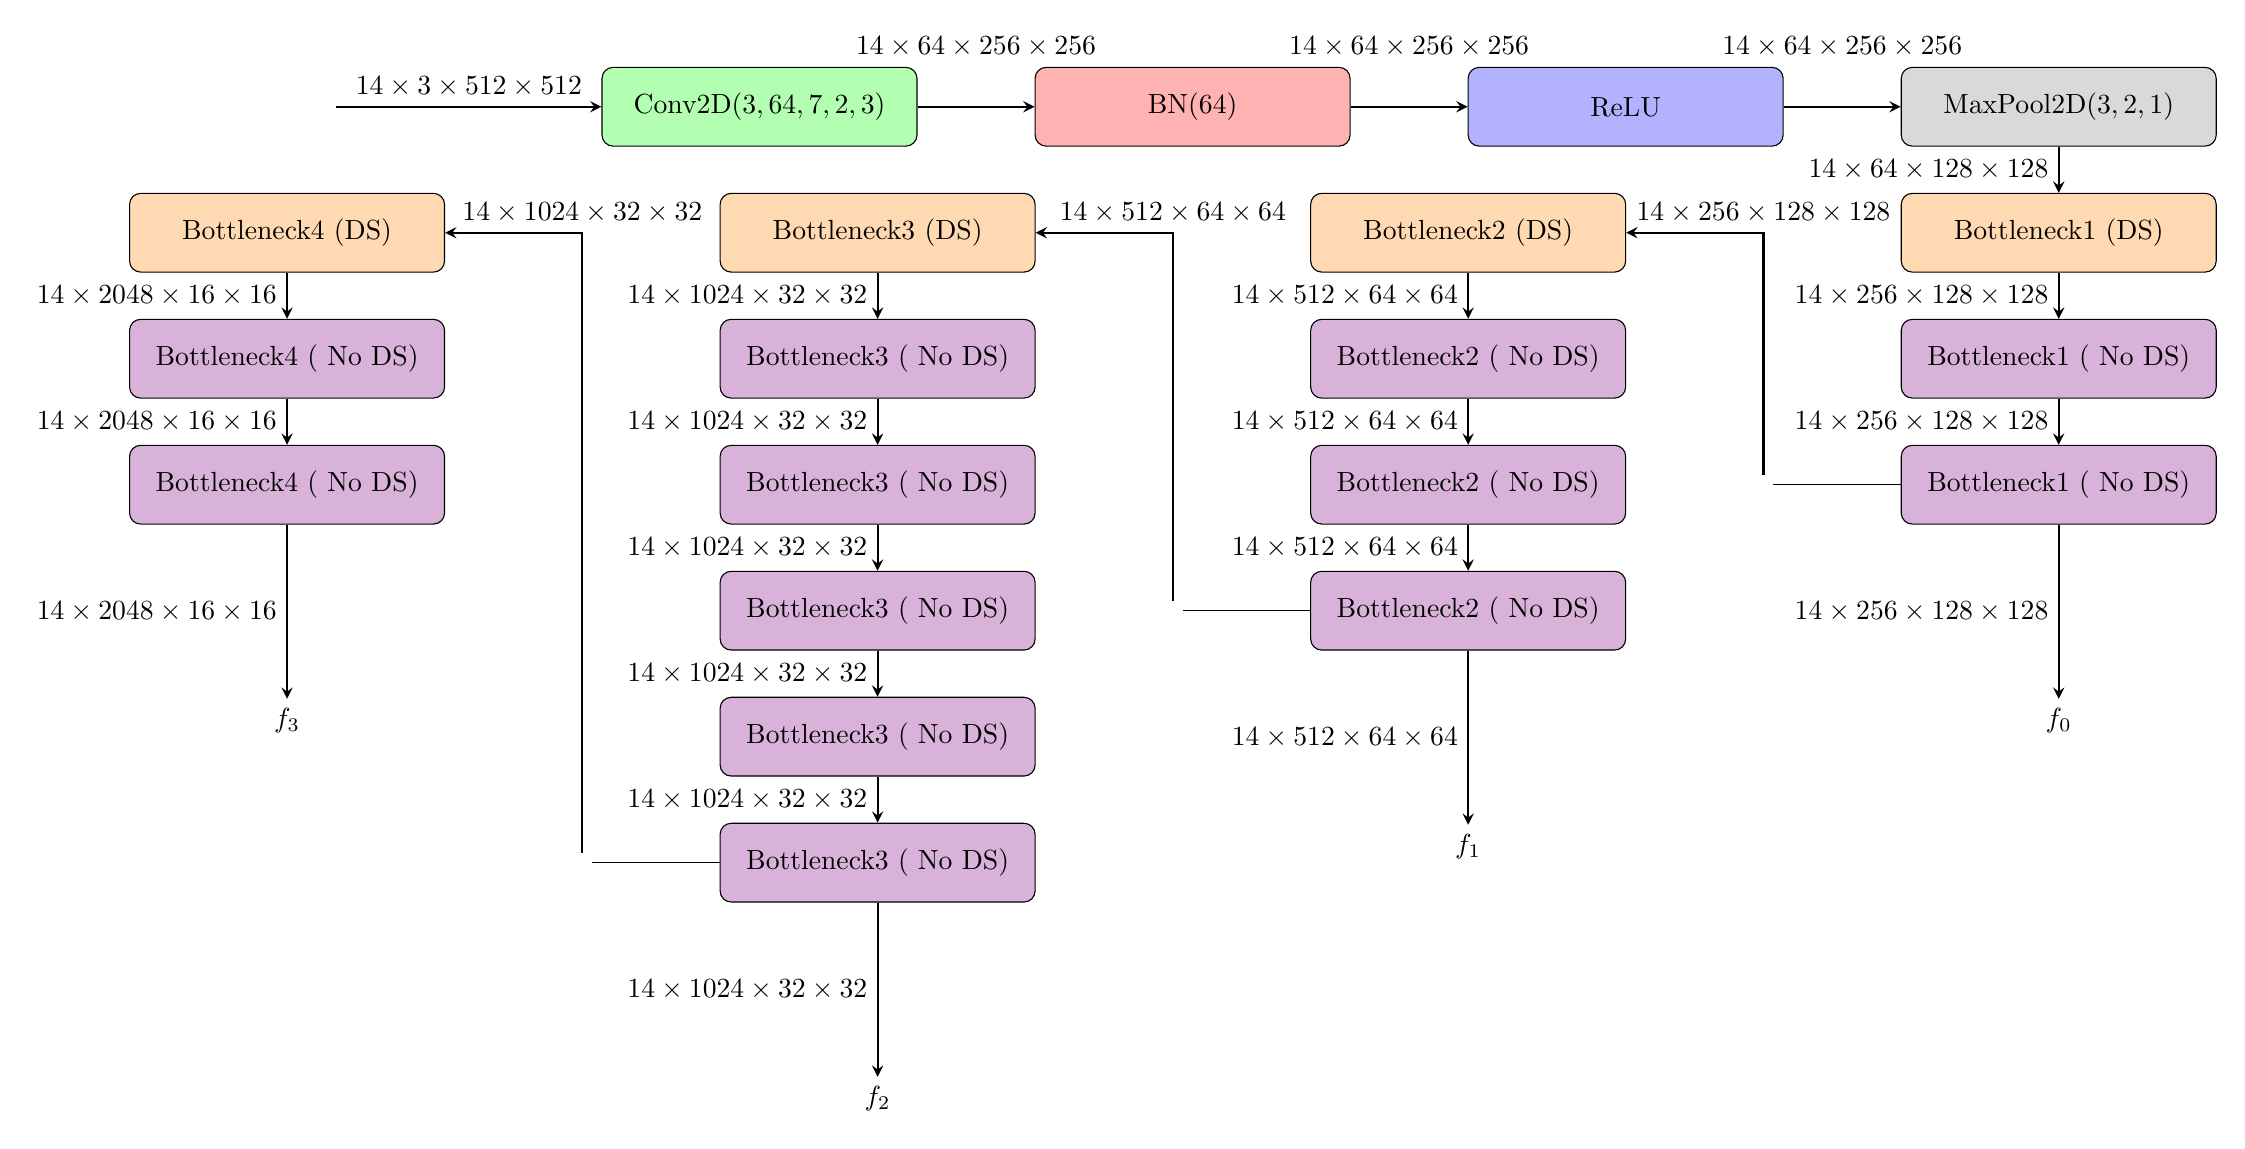
\begin{tikzpicture}[node distance=3cm]
\node (conv1) [conv2d, yshift=1 cm, xshift = -2.5cm] {Conv2D$(3, 64, 7, 2, 3)$};
\node (none) [left of= conv1, yshift=0 cm, xshift = -2.5cm] {};
\draw [arrow] (none) -- node[anchor=south] {$14 \times 3 \times 512 \times 512$} (conv1);

\node (bn1) [bn, right of=conv1, yshift=0, xshift = 2.5cm] {BN$(64)$};
\draw [arrow] (conv1) -- node[anchor=south, yshift=0.5 cm] {$14 \times 64 \times 256 \times 256$} (bn1);
\node (relu1) [relu, right of=bn1, yshift=0, xshift =2.5cm] {ReLU};
\draw [arrow] (bn1) -- node[anchor=south, yshift=0.5 cm] {$14 \times 64 \times 256 \times 256$} (relu1);
\node (maxpool1) [maxpool, right of=relu1, yshift=0, xshift = 2.5cm] {MaxPool2D($3,2,1$)};
\draw [arrow] (relu1) -- node[anchor=south, yshift=0.5 cm] {$14 \times 64 \times 256 \times 256$} (maxpool1);

\node (bt1_ds) [bt_ds, below of= maxpool1, yshift=\ttx cm, xshift = 0cm] {Bottleneck1 (DS)};
\draw [arrow] (maxpool1) -- node[anchor=east] {$14 \times 64 \times 128 \times 128$} (bt1_ds);

\node (bt1_nods1) [bt_nods, below of= bt1_ds , yshift=\ttx cm, xshift = 0cm] {Bottleneck1 ( No DS)};
\draw [arrow] (bt1_ds) -- node[anchor=east] {$14 \times 256  \times 128 \times 128$} (bt1_nods1);

\node (bt1_nods2) [bt_nods, below of= bt1_nods1 , yshift=\ttx cm, xshift = 0cm] {Bottleneck1 ( No DS)};
\draw [arrow] (bt1_nods1) -- node[anchor=east] {$14 \times 256 \times 128 \times 128$} (bt1_nods2);

\node (bt2_ds) [bt_ds, left of= bt1_ds, yshift=0 cm, xshift = -4.5cm] {Bottleneck2 (DS)};

\node (dummy1)  [left of= bt1_nods2, yshift=0 cm, xshift = -0.75 cm] {};
\draw (bt1_nods2) -- (dummy1);
\draw [arrow] (dummy1) |- node[anchor=south] {$14 \times 256  \times 128 \times 128$} (bt2_ds);

\node (bt2_nods1) [bt_nods, below of= bt2_ds , yshift=\ttx cm, xshift = 0cm] {Bottleneck2 ( No DS)};
\draw [arrow] (bt2_ds) -- node[anchor=east] {$14 \times 512  \times 64 \times 64$} (bt2_nods1);

\node (bt2_nods2) [bt_nods, below of= bt2_nods1 , yshift=\ttx cm, xshift = 0cm] {Bottleneck2 ( No DS)};
\draw [arrow] (bt2_nods1) -- node[anchor=east] {$14 \times 512 \times 64 \times 64$} (bt2_nods2);

\node (bt2_nods3) [bt_nods, below of= bt2_nods2 , yshift=\ttx cm, xshift = 0cm] {Bottleneck2 ( No DS)};
\draw [arrow] (bt2_nods2) -- node[anchor=east] {$14 \times 512 \times 64 \times 64$} (bt2_nods3);

\node (bt3_ds) [bt_ds, left of= bt2_ds, yshift=0 cm, xshift = -4.5cm] {Bottleneck3 (DS)};

\node (dummy2)  [left of= bt2_nods3, yshift=0 cm, xshift = -0.75 cm] {};
\draw (bt2_nods3) -- (dummy2);
\draw [arrow] (dummy2) |- node[anchor=south] {$14 \times 512  \times 64 \times 64$} (bt3_ds);

\node (bt3_nods1) [bt_nods, below of= bt3_ds , yshift=\ttx cm, xshift = 0cm] {Bottleneck3 ( No DS)};
\draw [arrow] (bt3_ds) -- node[anchor=east] {$14 \times 1024  \times 32 \times 32$} (bt3_nods1);

\node (bt3_nods2) [bt_nods, below of= bt3_nods1 , yshift=\ttx cm, xshift = 0cm] {Bottleneck3 ( No DS)};
\draw [arrow] (bt3_nods1) -- node[anchor=east] {$14 \times 1024  \times 32 \times 32$} (bt3_nods2);

\node (bt3_nods3) [bt_nods, below of= bt3_nods2 , yshift=\ttx cm, xshift = 0cm] {Bottleneck3 ( No DS)};
\draw [arrow] (bt3_nods2) -- node[anchor=east] {$14 \times 1024  \times 32 \times 32$} (bt3_nods3);

\node (bt3_nods4) [bt_nods, below of= bt3_nods3 , yshift=\ttx cm, xshift = 0cm] {Bottleneck3 ( No DS)};
\draw [arrow] (bt3_nods3) -- node[anchor=east] {$14 \times 1024  \times 32 \times 32$} (bt3_nods4);

\node (bt3_nods5) [bt_nods, below of= bt3_nods4 , yshift=\ttx cm, xshift = 0cm] {Bottleneck3 ( No DS)};
\draw [arrow] (bt3_nods4) -- node[anchor=east] {$14 \times 1024  \times 32 \times 32$} (bt3_nods5);

\node (bt4_ds) [bt_ds, left of= bt3_ds, yshift=0 cm, xshift = -4.5cm] {Bottleneck4 (DS)};

\node (dummy3)  [left of= bt3_nods5, yshift=0 cm, xshift = -0.75 cm] {};
\draw (bt3_nods5) -- (dummy3);
\draw [arrow] (dummy3) |- node[anchor=south] {$14 \times 1024  \times 32 \times 32$} (bt4_ds);

\node (bt4_nods1) [bt_nods, below of= bt4_ds , yshift=\ttx cm, xshift = 0cm] {Bottleneck4 ( No DS)};
\draw [arrow] (bt4_ds) -- node[anchor=east] {$14 \times 2048 \times 16 \times 16$} (bt4_nods1);

\node (bt4_nods2) [bt_nods, below of= bt4_nods1 , yshift=\ttx cm, xshift = 0cm] {Bottleneck4 ( No DS)};
\draw [arrow] (bt4_nods1) -- node[anchor=east] {$14 \times 2048 \times 16 \times 16$} (bt4_nods2);

\node (f0)  [below of= bt1_nods2, yshift=0 cm, xshift = 0 cm] {$f_0$};
\node (f1)  [below of= bt2_nods3, yshift=0 cm, xshift = 0 cm] {$f_1$};
\node (f2)  [below of= bt3_nods5, yshift=0 cm, xshift = 0 cm] {$f_2$};
\node (f3)  [below of= bt4_nods2, yshift=0 cm, xshift = 0 cm] {$f_3$};

\draw [arrow] (bt1_nods2) -- node[anchor=east] {$14 \times 256 \times 128 \times 128$} (f0);
\draw [arrow] (bt2_nods3) -- node[anchor=east] {$14 \times 512 \times 64 \times 64$} (f1);
\draw [arrow] (bt3_nods5) -- node[anchor=east] {$14 \times 1024  \times 32 \times 32$}(f2);
\draw [arrow] (bt4_nods2) -- node[anchor=east] {$14 \times 2048 \times 16 \times 16$}(f3);
\end{tikzpicture}
\caption{ResNet-50 architecture used.}
\label{fig_resnet}
\end{figure}



\begin{figure}
\centering
\begin{tikzpicture}[node distance=3cm]
\node (subtraction) [bt_ds, yshift=1 cm, xshift = -2.5cm] {Mean image subtraction};
\node (none) [left of= subtraction, yshift=0 cm, xshift = -2.5cm] {};
\draw [arrow] (none) -- node[anchor=south] {$14 \times 3 \times 512 \times 512$} (conv1);

\node (resnet) [maxpool, right of=subtraction, yshift=0, xshift = 4.5cm] {ResNet-50 Architecture};
\draw [arrow] (subtraction) -- node[anchor=south, yshift=0 cm] {$14 \times 3 \times 512 \times 512$} (resnet);

\node (f0_dum) [below of=resnet, yshift=1.5cm, xshift =4.5cm] {$f_0$};
\node (f1_dum) [left of=f0_dum, yshift=0cm, xshift =-4.5cm] {$f_1$};
\node (f2_dum) [left of=f1_dum, yshift=0cm, xshift =-4.5cm] {$f_2$};
\node (f3_dum) [left of=f2_dum, yshift=0cm, xshift =-4.5cm] {$f_3$};

\node (f0_next) [bt_ds, below of=resnet, yshift=0, xshift =4.5cm] {Concatenate};
\node (f1_next) [bt_ds, left of=f0_next, yshift=0, xshift =-4.5cm] {Concatenate};
\node (f2_next) [bt_ds, left of=f1_next, yshift=0, xshift =-4.5cm] {Concatenate};
\node (f3_next) [bt_ds, left of=f2_next, yshift=0, xshift =-4.5cm] {Upsample($2$, bilinear)};

\draw  (resnet) |- (f0_dum);
\draw  (resnet) |- (f1_dum);
\draw  (resnet) |- (f2_dum);
\draw  (resnet) |- (f3_dum);

\draw [arrow] (f0_dum) -- node[anchor=east, yshift=0 cm] {$14 \times 256 \times 128 \times 128$} (f0_next);
\draw [arrow] (f1_dum) -- node[anchor=east, yshift=0 cm] {$14 \times 512 \times 64 \times 64$} (f1_next);
\draw [arrow] (f2_dum) -- node[anchor=east, yshift=0 cm] {$14 \times 1024 \times 32 \times 32$} (f2_next);
\draw [arrow] (f3_dum) -- node[anchor=east, yshift=0 cm] {$14 \times 2048 \times 16 \times 16$} (f3_next);

\draw [arrow] (f3_next) -- node[anchor=south] {$14 \times 2048 \times 32 \times 32$} (f2_next);


\node (f2_conv1) [conv2d, below of= f2_next, yshift=\ttx cm, xshift = 0cm] {Conv2D$(3072, 128, 1)$};
\draw [arrow] (f2_next) -- node[anchor=east]  {$14 \times 3072 \times 32 \times 32$}  (f2_conv1);
\node (f2_bn1) [bn, below of= f2_conv1, yshift=\ttx cm, xshift = 0cm] {BN($128$)};
\draw [arrow] (f2_conv1) -- node[anchor=east]  {$14 \times 128 \times 32 \times 32$}  (f2_bn1);
\node (f2_relu1) [relu, below of= f2_bn1, yshift=\ttx cm, xshift = 0cm] {ReLU};
\draw [arrow] (f2_bn1) -- node[anchor=east]  {$14 \times 128 \times 32 \times 32$}  (f2_relu1);

\node (f2_conv2) [conv2d,  below of= f2_relu1, yshift=\ttx cm, xshift = 0cm] {Conv2D$(128, 128, 3,1,1)$};
\draw [arrow] (f2_relu1) -- node[anchor=east]  {$14 \times 128 \times 32 \times 32$}  (f2_conv2);
\node (f2_bn2) [bn, below of= f2_conv2, yshift=\ttx cm, xshift = 0cm] {BN($128$)};
\draw [arrow] (f2_conv2) -- node[anchor=east]  {$14 \times 128 \times 32 \times 32$}  (f2_bn2);
\node (f2_relu2) [relu, below of= f2_bn2, yshift=\ttx cm, xshift = 0cm] {ReLU};
\draw [arrow] (f2_bn2) -- node[anchor=east]  {$14 \times 128 \times 32 \times 32$}  (f2_relu2);

\node (f2_upsample) [bt_ds, below of=f2_bn2, yshift=0, xshift =-0] {Upsample($2$, bilinear)};
\draw [arrow] (f2_relu2) -- node[anchor=east]  {$14 \times 128 \times 32 \times 32$}  (f2_upsample);

\node (f2_dom) [right of=f2_upsample, yshift=0, xshift =0cm]{};
\draw (f2_upsample) -- (f2_dom);
\draw [arrow] (f2_dom) |- node[anchor=south, xshift = 0.7cm] {$14 \times 128 \times 64 \times 64$} (f1_next);



\node (f1_conv1) [conv2d, below of= f1_next, yshift=\ttx cm, xshift = 0cm] {Conv2D$(640, 64, 1)$};
\draw [arrow] (f1_next) -- node[anchor=east]  {$14 \times 640 \times 64 \times 64$}  (f1_conv1);
\node (f1_bn1) [bn, below of= f1_conv1, yshift=\ttx cm, xshift = 0cm] {BN($64$)};
\draw [arrow] (f1_conv1) -- node[anchor=east]  {$14 \times 64 \times 64 \times 64$}  (f1_bn1);
\node (f1_relu1) [relu, below of= f1_bn1, yshift=\ttx cm, xshift = 0cm] {ReLU};
\draw [arrow] (f1_bn1) -- node[anchor=east]  {$14 \times 64 \times 64 \times 64$}  (f1_relu1);

\node (f1_conv2) [conv2d,  below of= f1_relu1, yshift=\ttx cm, xshift = 0cm] {Conv2D$(64, 64, 3,1,1)$};
\draw [arrow] (f1_relu1) -- node[anchor=east]  {$14 \times 64 \times 64 \times 64$}  (f1_conv2);
\node (f1_bn2) [bn, below of= f1_conv2, yshift=\ttx cm, xshift = 0cm] {BN($64$)};
\draw [arrow] (f1_conv2) -- node[anchor=east]  {$14 \times 64 \times 64 \times 64$}  (f1_bn2);
\node (f1_relu2) [relu, below of= f1_bn2, yshift=\ttx cm, xshift = 0cm] {ReLU};
\draw [arrow] (f1_bn2) -- node[anchor=east]  {$14 \times 64 \times 64 \times 64$}  (f1_relu2);

\node (f1_upsample) [bt_ds, below of=f1_bn2, yshift=0, xshift =-0] {Upsample($2$, bilinear)};
\draw [arrow] (f1_relu2) -- node[anchor=east]  {$14 \times 64 \times 64 \times 64$}  (f1_upsample);

\node (f1_dom) [right of=f1_upsample, yshift=0, xshift =0cm]{};
\draw (f1_upsample) -- (f1_dom);
\draw [arrow] (f1_dom) |- node[anchor=south, xshift = 0.7cm] {$14 \times 64 \times 128 \times 128$} (f0_next);


\node (f0_conv1) [conv2d, below of= f0_next, yshift=\ttx cm, xshift = 0cm] {Conv2D$(320, 64, 1)$};
\draw [arrow] (f0_next) -- node[anchor=east]  {$14 \times 320 \times 128 \times 128$}  (f0_conv1);
\node (f0_bn1) [bn, below of= f0_conv1, yshift=\ttx cm, xshift = 0cm] {BN($64$)};
\draw [arrow] (f0_conv1) -- node[anchor=east]  {$14 \times 64 \times 128 \times 128$}  (f0_bn1);
\node (f0_relu1) [relu, below of= f0_bn1, yshift=\ttx cm, xshift = 0cm] {ReLU};
\draw [arrow] (f0_bn1) -- node[anchor=east]  {$14 \times 64 \times 128 \times 128$}  (f0_relu1);

\node (f0_conv2) [conv2d,  below of= f0_relu1, yshift=\ttx cm, xshift = 0cm] {Conv2D$(64, 32, 3,1,1)$};
\draw [arrow] (f0_relu1) -- node[anchor=east]  {$14 \times 64 \times 128 \times 128$}  (f0_conv2);
\node (f0_bn2) [bn, below of= f0_conv2, yshift=\ttx cm, xshift = 0cm] {BN($32$)};
\draw [arrow] (f0_conv2) -- node[anchor=east]  {$14 \times 32 \times 128 \times 128$}  (f0_bn2);
\node (f0_relu2) [relu, below of= f0_bn2, yshift=\ttx cm, xshift = 0cm] {ReLU};
\draw [arrow] (f0_bn2) -- node[anchor=east]  {$14 \times 32 \times 128 \times 128$}  (f0_relu2);

\node (f0_dom) [below of=f0_relu2, yshift=0, xshift =0cm]{};
\draw  [arrow] (f0_relu2) -- node[anchor=east]  {$14 \times 32 \times 128 \times 128$} (f0_dom) ;
\end{tikzpicture}
\caption{Architecture to concatenate ResNet outputs.}
\label{fig_overall}
\end{figure}


\begin{figure}
\centering
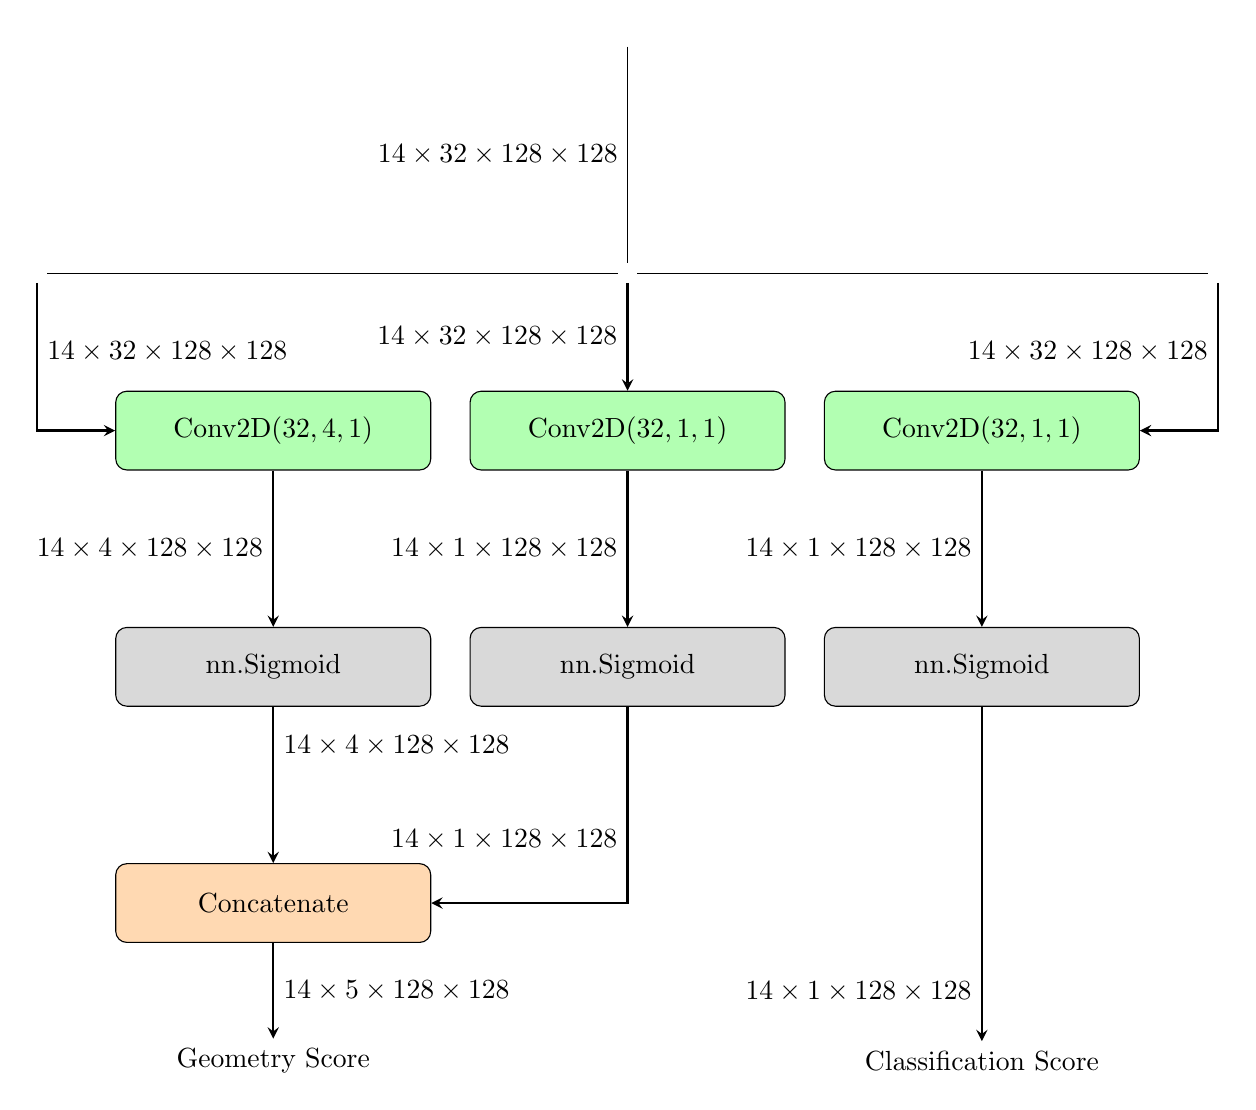
\begin{tikzpicture}[node distance=3cm]
\node (none0) [yshift=0 cm, xshift = 0cm] {};
\node (none1) [below of=none0, yshift=0 cm, xshift = 0cm] {};
\node (none2) [right of=none1, yshift=0 cm, xshift = 4.5cm] {};
\node (none3) [left of=none1, yshift=0 cm, xshift = -4.5cm] {};
\draw  (none0) -- node[anchor=east, yshift=0 cm] {$14 \times 32 \times 128 \times 128$} (none1);
\draw  (none1) --  (none2);
\draw  (none1) --  (none3);

\node (conv1) [conv2d, below of =none1, yshift=1 cm, xshift = 0cm] {Conv2D$(32,1,1)$};
\node (conv2) [conv2d, below of =none1, yshift=1 cm, xshift = 4.5cm] {Conv2D$(32,1,1)$};
\node (conv3) [conv2d, below of =none1, yshift=1 cm, xshift = -4.5cm] {Conv2D$(32,4,1)$};

\draw [arrow] (none2) |- node[anchor=east, yshift = 1cm] {$14 \times 32 \times 128 \times 128$} (conv2);
\draw [arrow] (none1) -- node[anchor=east] {$14 \times 32 \times 128 \times 128$} (conv1);
\draw [arrow] (none3) |- node[anchor=west, yshift = 1cm] {$14 \times 32 \times 128 \times 128$} (conv3);

\node (s1) [maxpool, below of =conv1, yshift=0 cm, xshift = 0cm] {nn.Sigmoid};
\node (s2) [maxpool, below of =conv2, yshift=0 cm, xshift = 0cm] {nn.Sigmoid};
\node (s3) [maxpool, below of =conv3, yshift=0 cm, xshift = 0cm] {nn.Sigmoid};
\node (geo) [bt_ds, below of =s3, yshift=0 cm, xshift = 0cm] {Concatenate};
\node (fscore) [below of =s2, yshift=-2 cm, xshift = 0cm] {Classification Score};
\node (fgeometry) [below of =geo, yshift=1 cm, xshift = 0cm] {Geometry Score};

\draw [arrow] (conv1) -- node[anchor=east, yshift = 0cm] {$14 \times 1 \times 128 \times 128$} (s1);
\draw [arrow] (conv2) -- node[anchor=east, yshift = 0cm] {$14 \times 1 \times 128 \times 128$} (s2);
\draw [arrow] (conv3) -- node[anchor=east, yshift = 0cm] {$14 \times 4 \times 128 \times 128$} (s3);

\draw [arrow] (s2) -- node[anchor=east, yshift = -1.5cm] {$14 \times 1 \times 128 \times 128$} (fscore);
\draw [arrow] (s1) |- node[anchor=east, yshift = 0.8cm] {$14 \times 1 \times 128 \times 128$} (geo);
\draw [arrow] (s3) -- node[anchor=west, yshift = 0.5cm] {$14 \times 4 \times 128 \times 128$} (geo);
\draw [arrow] (geo) -- node[anchor=west, yshift = 0cm] {$14 \times 5 \times 128 \times 128$} (fgeometry);

\end{tikzpicture}
\caption{Final network layers.}
\label{fig_final}
\end{figure}
\begin{figure}
\centering
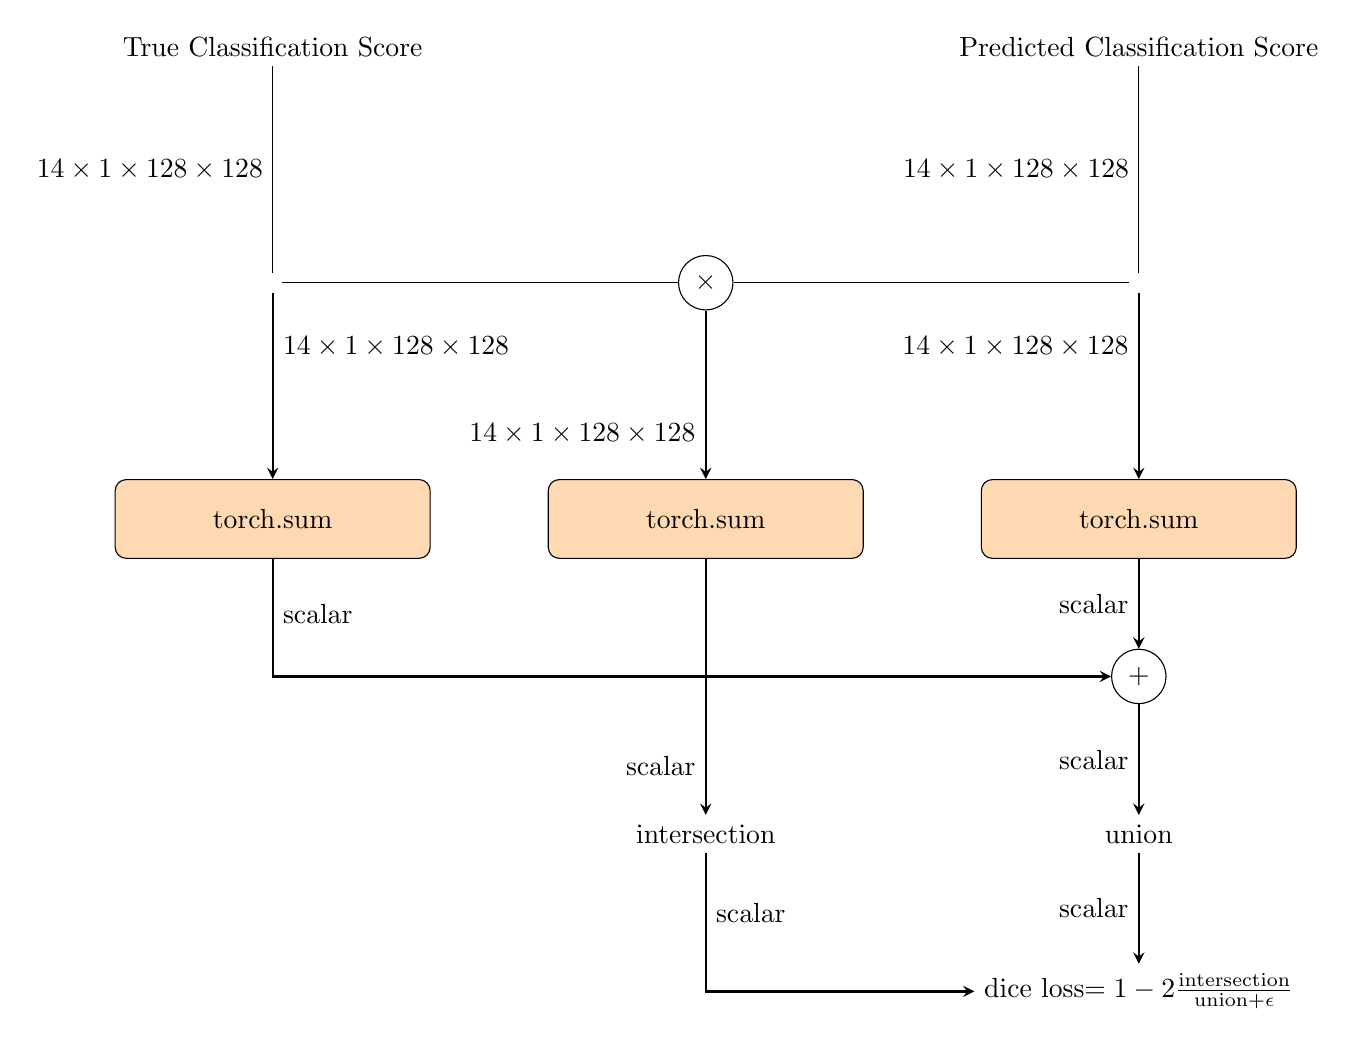
\begin{tikzpicture}[node distance=3cm]
\node (none0) [yshift=0 cm, xshift = 0cm] {Predicted Classification Score};
\node (none1) [left of=none0, yshift=0 cm, xshift = -8cm] {True Classification Score};

\node (none2) [below of=none0, yshift=0 cm, xshift =0cm] {};
\node (none3) [below of=none1, yshift=0 cm, xshift = 0cm] {};

\node (none4) [add, left of=none2, yshift=0 cm, xshift =-2.5cm] {$\times$};
\node (none5) [right of=none3, yshift=0 cm, xshift = 2.5cm] {};

\node (none6) [below of=none0, yshift=0 cm, xshift =0cm] {};
\node (none7) [below of=none1, yshift=0 cm, xshift = 0cm] {};

\draw (none0) -- node[anchor=east, yshift=0 cm] {$14 \times 1 \times 128 \times 128$} (none2);
\draw  (none1) -- node[anchor=east, yshift=0 cm] {$14 \times 1 \times 128 \times 128$} (none3);

\draw (none2) --   (none4);
\draw  (none3) --   (none4);


\node (sumpred) [bt_ds, below of = none2, yshift=0 cm, xshift = 0cm] {torch.sum};
\node (sumtrue) [bt_ds, below of =none3, yshift=0 cm, xshift = 0cm] {torch.sum};
\node (prodd) [bt_ds, below of =none4, yshift=0 cm, xshift = 0cm] {torch.sum};

\draw  [arrow](none2) --  node[anchor=east, yshift=0.5 cm] {$14 \times 1 \times 128 \times 128$} (sumpred);
\draw  [arrow](none3) --  node[anchor=west, yshift=0.5 cm] {$14 \times 1 \times 128 \times 128$} (sumtrue);
\draw  [arrow](none4) --  node[anchor=east, yshift=-0.5 cm] {$14 \times 1 \times 128 \times 128$} (prodd);

\node (none5) [add, below of=sumpred, yshift=1 cm, xshift =0cm] {$+$};
\draw  [arrow](sumtrue) |-  node[anchor=west, yshift=0.8 cm] {scalar} (none5);
\draw  [arrow](sumpred) --  node[anchor=east, yshift=0 cm] {scalar} (none5);

\node (none6) [ below of=prodd, yshift=-1 cm, xshift =0cm] {intersection};
\draw  [arrow](prodd) --  node[anchor=east, yshift=-1 cm] {scalar} (none6);

\node (none7) [ below of=none5, yshift=1 cm, xshift =0cm] {union};
\draw  [arrow](none5) --  node[anchor=east, yshift=0 cm] {scalar} (none7);

\node (none8) [ below of=none7, yshift=1 cm, xshift =0cm] {dice loss$=1-2\frac{\textrm{intersection}}{\textrm{union} + \epsilon}$ };
\draw  [arrow](none7) --  node[anchor=east, yshift=0 cm] {scalar} (none8);
\draw  [arrow](none6) |-  node[anchor=west, yshift=1 cm] {scalar} (none8);
\end{tikzpicture}
\caption{Dice loss calculation}
\label{fig_dice_loss}
\end{figure}

\newpage
\section{Loss}
\subsection{Geometry loss calculation}
Both predicted and true Geometry Score tensors of size $14 \times 5 \times 128 \times 128$ are split into 4 tensors each with sizes $14 \times 1 \times 128 \times 128$. These tensors are respectively called $d^1_{gt}, d^2_{gt}, d^3_{gt}, d^4_{gt}, {\theta}_{gt}$ and $d^1_{pr}, d^2_{pr}, d^3_{pr}, d^4_{pr}, {\theta}_{pr}$. Then the following element-wise operations are done to find tensors $\textrm{Area}_{gt}$ and $\textrm{Area}_{pr}$ of sizes $14 \times 1 \times 128 \times 128$,
\begin{align}
\textrm{Area}_{gt} &= (d^1_{gt} + d^3_{gt}) \odot  (d^2_{gt} + d^4_{gt}) \\
\textrm{Area}_{pr} &= (d^1_{pr} + d^3_{pr}) \odot  (d^2_{pr} + d^4_{pr}).
\end{align}
To find the intersection area tensor, the following element-wise tensor operations are used  which result is tensors $w_{\textrm{union}}$ and $h_{\textrm{union}}$ of sizes $14 \times 1 \times 128 \times 128$, 
\begin{align}
w_{\textrm{union}} &= \min (d^2_{gt}, d^2_{pr}) + \min ( d^4_{gt}, d^4_{pr})  \\
h_{\textrm{union}} &= \min (d^1_{gt}, d^1_{pr}) + \min ( d^3_{gt}, d^3_{pr}). 
\end{align}
This allows us to compute the area intersection and union tensors  of size $14 \times 1 \times 128 \times 128$ as follows,
\begin{align}
\textrm{Area}_{\textrm{intersection}} &= w_{\textrm{union}} \odot h_{\textrm{union}} \\
\textrm{Area}_{\textrm{union}} &= 
\textrm{Area}_{gt} + \textrm{Area}_{pr} -
\textrm{Area}_{\textrm{intersection}}.
\end{align}
Using these areas and based on element-wise tensor operations, the loss tensor $L_{\textrm{AABB}}$ of  size $14 \times 1 \times 128 \times 128$ is calculated as follows,
\begin{align}
L_{\textrm{AABB}} = - \log \left( \frac{\textrm{Area}_{\textrm{intersection}} + 1}{ \textrm{Area}_{\textrm{union}}+ 1}\right).
\end{align}
The angle loss tensor $L_{\theta}$ and the overall loss tensor $L_g$ of sizes $14 \times 1 \times 128 \times 128$ are also calculated as follows,
\begin{align}
L_{\theta} &= 1 - \cos \left( \theta_{pr} - \theta_{tr} \right) \\
L_{g} &= L_{\textrm{AABB}}  + 20 L_{\theta}.
\end{align}
Finally, the overall loss value is calculates as 
\begin{align}
l = \textrm{torch.mean}( L_g \odot y_{tr}) + L_{\textrm{classification}} 
\end{align}
\end{document}
